% Created by tikzDevice version 0.12.3 on 2020-07-22 15:14:14
% !TEX encoding = UTF-8 Unicode
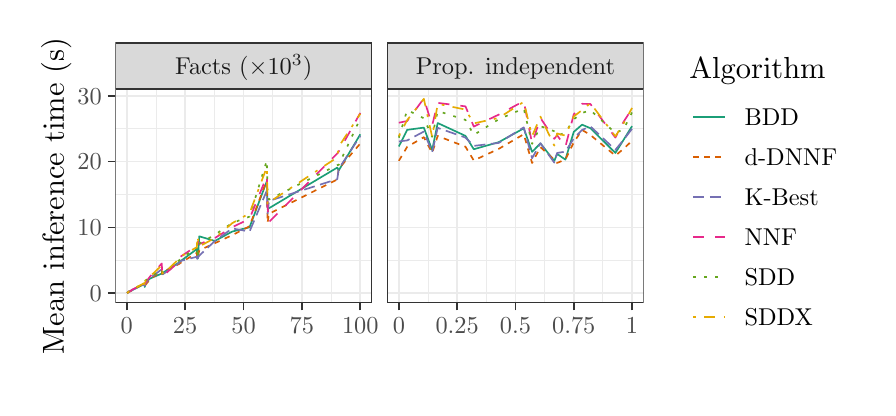
\begin{tikzpicture}[x=1pt,y=1pt]
\definecolor{fillColor}{RGB}{255,255,255}
\path[use as bounding box,fill=fillColor,fill opacity=0.00] (0,0) rectangle (303.53,130.09);
\begin{scope}
\path[clip] (  0.00,  0.00) rectangle (303.53,130.09);
\definecolor{drawColor}{RGB}{255,255,255}
\definecolor{fillColor}{RGB}{255,255,255}

\path[draw=drawColor,line width= 0.6pt,line join=round,line cap=round,fill=fillColor] (  0.00,  0.00) rectangle (303.53,130.09);
\end{scope}
\begin{scope}
\path[clip] ( 31.71, 30.69) rectangle (124.41,108.01);
\definecolor{fillColor}{RGB}{255,255,255}

\path[fill=fillColor] ( 31.71, 30.69) rectangle (124.41,108.01);
\definecolor{drawColor}{gray}{0.92}

\path[draw=drawColor,line width= 0.3pt,line join=round] ( 31.71, 46.03) --
	(124.41, 46.03);

\path[draw=drawColor,line width= 0.3pt,line join=round] ( 31.71, 69.81) --
	(124.41, 69.81);

\path[draw=drawColor,line width= 0.3pt,line join=round] ( 31.71, 93.59) --
	(124.41, 93.59);

\path[draw=drawColor,line width= 0.3pt,line join=round] ( 46.35, 30.69) --
	( 46.35,108.01);

\path[draw=drawColor,line width= 0.3pt,line join=round] ( 67.45, 30.69) --
	( 67.45,108.01);

\path[draw=drawColor,line width= 0.3pt,line join=round] ( 88.54, 30.69) --
	( 88.54,108.01);

\path[draw=drawColor,line width= 0.3pt,line join=round] (109.64, 30.69) --
	(109.64,108.01);

\path[draw=drawColor,line width= 0.6pt,line join=round] ( 31.71, 34.14) --
	(124.41, 34.14);

\path[draw=drawColor,line width= 0.6pt,line join=round] ( 31.71, 57.92) --
	(124.41, 57.92);

\path[draw=drawColor,line width= 0.6pt,line join=round] ( 31.71, 81.70) --
	(124.41, 81.70);

\path[draw=drawColor,line width= 0.6pt,line join=round] ( 31.71,105.48) --
	(124.41,105.48);

\path[draw=drawColor,line width= 0.6pt,line join=round] ( 35.80, 30.69) --
	( 35.80,108.01);

\path[draw=drawColor,line width= 0.6pt,line join=round] ( 56.90, 30.69) --
	( 56.90,108.01);

\path[draw=drawColor,line width= 0.6pt,line join=round] ( 78.00, 30.69) --
	( 78.00,108.01);

\path[draw=drawColor,line width= 0.6pt,line join=round] ( 99.09, 30.69) --
	( 99.09,108.01);

\path[draw=drawColor,line width= 0.6pt,line join=round] (120.19, 30.69) --
	(120.19,108.01);
\definecolor{drawColor}{RGB}{27,158,119}

\path[draw=drawColor,line width= 0.6pt,line join=round] ( 35.93, 34.22) --
	( 36.05, 34.28) --
	( 36.31, 34.45) --
	( 36.64, 34.74) --
	( 36.81, 34.74) --
	( 37.82, 35.27) --
	( 42.19, 37.45) --
	( 42.32, 36.38) --
	( 42.57, 37.84) --
	( 44.24, 39.46) --
	( 48.46, 41.24) --
	( 48.58, 41.31) --
	( 48.84, 41.51) --
	( 54.85, 45.33) --
	( 55.10, 45.62) --
	( 61.12, 50.08) --
	( 61.24, 47.64) --
	( 61.37, 50.15) --
	( 61.50, 46.59) --
	( 62.00, 54.70) --
	( 67.64, 53.02) --
	( 73.90, 56.41) --
	( 80.17, 57.95) --
	( 86.43, 74.63) --
	( 86.69, 65.78) --
	( 87.19, 64.84) --
	(111.88, 79.54) --
	(112.39, 78.48) --
	(120.19, 91.54);
\definecolor{drawColor}{RGB}{217,95,2}

\path[draw=drawColor,line width= 0.6pt,dash pattern=on 2pt off 2pt ,line join=round] ( 35.93, 34.20) --
	( 36.05, 34.26) --
	( 36.31, 34.41) --
	( 36.64, 34.70) --
	( 36.81, 34.68) --
	( 37.82, 35.23) --
	( 42.19, 37.74) --
	( 42.32, 37.05) --
	( 42.57, 37.14) --
	( 44.24, 39.19) --
	( 48.46, 42.35) --
	( 48.58, 40.98) --
	( 48.84, 41.86) --
	( 54.85, 44.75) --
	( 55.10, 45.01) --
	( 61.12, 48.70) --
	( 61.24, 46.51) --
	( 61.37, 47.05) --
	( 61.50, 47.32) --
	( 62.00, 49.64) --
	( 67.64, 52.22) --
	( 73.90, 55.11) --
	( 80.17, 58.33) --
	( 86.43, 75.16) --
	( 86.69, 59.59) --
	( 87.19, 62.82) --
	(111.88, 75.24) --
	(112.39, 79.11) --
	(120.19, 88.23);
\definecolor{drawColor}{RGB}{117,112,179}

\path[draw=drawColor,line width= 0.6pt,dash pattern=on 4pt off 2pt ,line join=round] ( 35.93, 34.22) --
	( 36.05, 34.33) --
	( 36.31, 34.49) --
	( 36.64, 34.77) --
	( 36.81, 34.77) --
	( 37.82, 35.37) --
	( 42.19, 37.40) --
	( 42.32, 36.84) --
	( 42.57, 37.68) --
	( 44.24, 39.58) --
	( 48.46, 42.81) --
	( 48.58, 41.77) --
	( 48.84, 40.98) --
	( 54.85, 45.16) --
	( 55.10, 45.74) --
	( 61.12, 47.31) --
	( 61.24, 46.52) --
	( 61.37, 48.59) --
	( 61.50, 46.96) --
	( 62.00, 47.72) --
	( 67.64, 52.99) --
	( 73.90, 57.55) --
	( 80.17, 56.42) --
	( 86.43, 71.23) --
	( 86.69, 62.93) --
	( 87.19, 67.49) --
	(111.88, 75.36) --
	(112.39, 79.09) --
	(120.19, 90.92);
\definecolor{drawColor}{RGB}{231,41,138}

\path[draw=drawColor,line width= 0.6pt,dash pattern=on 4pt off 4pt ,line join=round] ( 35.93, 34.22) --
	( 36.05, 34.29) --
	( 36.31, 34.48) --
	( 36.64, 34.79) --
	( 36.81, 34.74) --
	( 37.82, 35.45) --
	( 42.19, 37.64) --
	( 42.32, 37.18) --
	( 42.57, 37.98) --
	( 44.24, 40.20) --
	( 48.46, 44.88) --
	( 48.58, 42.06) --
	( 48.84, 40.35) --
	( 54.85, 45.65) --
	( 55.10, 47.25) --
	( 61.12, 51.25) --
	( 61.24, 51.16) --
	( 61.37, 51.25) --
	( 61.50, 52.79) --
	( 62.00, 51.87) --
	( 67.64, 54.08) --
	( 73.90, 57.97) --
	( 80.17, 61.03) --
	( 86.43, 76.47) --
	( 86.69, 65.20) --
	( 87.19, 59.83) --
	(111.88, 84.66) --
	(112.39, 85.31) --
	(120.19, 99.29);
\definecolor{drawColor}{RGB}{102,166,30}

\path[draw=drawColor,line width= 0.6pt,dash pattern=on 1pt off 3pt ,line join=round] ( 35.93, 34.24) --
	( 36.05, 34.31) --
	( 36.31, 34.48) --
	( 36.64, 34.81) --
	( 36.81, 34.77) --
	( 37.82, 35.45) --
	( 42.19, 37.88) --
	( 42.32, 38.54) --
	( 42.57, 38.69) --
	( 44.24, 39.95) --
	( 48.46, 42.70) --
	( 48.58, 41.93) --
	( 48.84, 41.20) --
	( 54.85, 46.14) --
	( 55.10, 46.43) --
	( 61.12, 50.70) --
	( 61.24, 47.87) --
	( 61.37, 50.28) --
	( 61.50, 47.98) --
	( 62.00, 52.07) --
	( 67.64, 55.24) --
	( 73.90, 59.51) --
	( 80.17, 61.81) --
	( 86.43, 82.15) --
	( 86.69, 68.77) --
	( 87.19, 67.98) --
	(111.88, 80.43) --
	(112.39, 80.51) --
	(120.19, 97.30);
\definecolor{drawColor}{RGB}{230,171,2}

\path[draw=drawColor,line width= 0.6pt,dash pattern=on 1pt off 3pt on 4pt off 3pt ,line join=round] ( 35.93, 34.20) --
	( 36.05, 34.32) --
	( 36.31, 34.47) --
	( 36.64, 34.80) --
	( 36.81, 34.78) --
	( 37.82, 35.44) --
	( 42.19, 37.83) --
	( 42.32, 36.07) --
	( 42.57, 38.73) --
	( 44.24, 40.20) --
	( 48.46, 44.23) --
	( 48.58, 43.29) --
	( 48.84, 40.97) --
	( 54.85, 46.70) --
	( 55.10, 47.28) --
	( 61.12, 50.76) --
	( 61.24, 52.81) --
	( 61.37, 51.86) --
	( 61.50, 53.84) --
	( 62.00, 51.03) --
	( 67.64, 54.08) --
	( 73.90, 59.44) --
	( 80.17, 63.01) --
	( 86.43, 79.72) --
	( 86.69, 66.18) --
	( 87.19, 66.97) --
	(111.88, 83.22) --
	(112.39, 87.08) --
	(120.19, 98.99);
\definecolor{drawColor}{gray}{0.20}

\path[draw=drawColor,line width= 0.6pt,line join=round,line cap=round] ( 31.71, 30.69) rectangle (124.41,108.01);
\end{scope}
\begin{scope}
\path[clip] (129.91, 30.69) rectangle (222.60,108.01);
\definecolor{fillColor}{RGB}{255,255,255}

\path[fill=fillColor] (129.91, 30.69) rectangle (222.60,108.01);
\definecolor{drawColor}{gray}{0.92}

\path[draw=drawColor,line width= 0.3pt,line join=round] (129.91, 46.03) --
	(222.60, 46.03);

\path[draw=drawColor,line width= 0.3pt,line join=round] (129.91, 69.81) --
	(222.60, 69.81);

\path[draw=drawColor,line width= 0.3pt,line join=round] (129.91, 93.59) --
	(222.60, 93.59);

\path[draw=drawColor,line width= 0.3pt,line join=round] (144.65, 30.69) --
	(144.65,108.01);

\path[draw=drawColor,line width= 0.3pt,line join=round] (165.72, 30.69) --
	(165.72,108.01);

\path[draw=drawColor,line width= 0.3pt,line join=round] (186.79, 30.69) --
	(186.79,108.01);

\path[draw=drawColor,line width= 0.3pt,line join=round] (207.85, 30.69) --
	(207.85,108.01);

\path[draw=drawColor,line width= 0.6pt,line join=round] (129.91, 34.14) --
	(222.60, 34.14);

\path[draw=drawColor,line width= 0.6pt,line join=round] (129.91, 57.92) --
	(222.60, 57.92);

\path[draw=drawColor,line width= 0.6pt,line join=round] (129.91, 81.70) --
	(222.60, 81.70);

\path[draw=drawColor,line width= 0.6pt,line join=round] (129.91,105.48) --
	(222.60,105.48);

\path[draw=drawColor,line width= 0.6pt,line join=round] (134.12, 30.69) --
	(134.12,108.01);

\path[draw=drawColor,line width= 0.6pt,line join=round] (155.19, 30.69) --
	(155.19,108.01);

\path[draw=drawColor,line width= 0.6pt,line join=round] (176.25, 30.69) --
	(176.25,108.01);

\path[draw=drawColor,line width= 0.6pt,line join=round] (197.32, 30.69) --
	(197.32,108.01);

\path[draw=drawColor,line width= 0.6pt,line join=round] (218.39, 30.69) --
	(218.39,108.01);
\definecolor{drawColor}{RGB}{27,158,119}

\path[draw=drawColor,line width= 0.6pt,line join=round] (134.12, 87.17) --
	(137.13, 93.17) --
	(143.15, 93.97) --
	(146.16, 85.86) --
	(148.16, 95.63) --
	(158.20, 90.99) --
	(161.20, 86.16) --
	(170.23, 88.72) --
	(179.26, 93.71) --
	(182.27, 85.21) --
	(185.28, 88.26) --
	(190.30, 81.94) --
	(191.30, 84.46) --
	(194.31, 82.43) --
	(197.32, 92.42) --
	(200.33, 95.04) --
	(203.34, 93.76) --
	(212.37, 84.82) --
	(215.38, 89.64) --
	(218.39, 94.51);
\definecolor{drawColor}{RGB}{217,95,2}

\path[draw=drawColor,line width= 0.6pt,dash pattern=on 2pt off 2pt ,line join=round] (134.12, 81.98) --
	(137.13, 87.03) --
	(143.15, 90.51) --
	(146.16, 84.86) --
	(148.16, 90.95) --
	(158.20, 87.07) --
	(161.20, 82.10) --
	(170.23, 86.31) --
	(179.26, 91.58) --
	(182.27, 81.17) --
	(185.28, 86.92) --
	(190.30, 82.36) --
	(191.30, 81.20) --
	(194.31, 82.46) --
	(197.32, 88.61) --
	(200.33, 93.14) --
	(203.34, 91.31) --
	(212.37, 83.85) --
	(215.38, 86.37) --
	(218.39, 89.25);
\definecolor{drawColor}{RGB}{117,112,179}

\path[draw=drawColor,line width= 0.6pt,dash pattern=on 4pt off 2pt ,line join=round] (134.12, 88.97) --
	(137.13, 89.35) --
	(143.15, 92.54) --
	(146.16, 85.10) --
	(148.16, 93.89) --
	(158.20, 90.38) --
	(161.20, 87.37) --
	(170.23, 88.45) --
	(179.26, 94.07) --
	(182.27, 82.90) --
	(185.28, 88.35) --
	(190.30, 81.32) --
	(191.30, 84.81) --
	(194.31, 85.30) --
	(197.32, 90.02) --
	(200.33, 93.14) --
	(203.34, 94.41) --
	(212.37, 85.94) --
	(215.38, 89.62) --
	(218.39, 93.56);
\definecolor{drawColor}{RGB}{231,41,138}

\path[draw=drawColor,line width= 0.6pt,dash pattern=on 4pt off 4pt ,line join=round] (134.12, 95.74) --
	(137.13, 96.35) --
	(143.15,104.50) --
	(146.16, 94.79) --
	(148.16,102.91) --
	(158.20,101.65) --
	(161.20, 94.35) --
	(170.23, 98.68) --
	(179.26,103.55) --
	(182.27, 88.20) --
	(185.28, 97.47) --
	(190.30, 89.92) --
	(191.30, 91.22) --
	(194.31, 87.06) --
	(197.32, 98.75) --
	(200.33,102.58) --
	(203.34,102.50) --
	(212.37, 90.37) --
	(215.38, 96.15) --
	(218.39,100.82);
\definecolor{drawColor}{RGB}{102,166,30}

\path[draw=drawColor,line width= 0.6pt,dash pattern=on 1pt off 3pt ,line join=round] (134.12, 90.34) --
	(137.13,100.33) --
	(143.15, 97.34) --
	(146.16, 90.63) --
	(148.16, 99.99) --
	(158.20, 96.75) --
	(161.20, 91.32) --
	(170.23, 97.00) --
	(179.26,100.90) --
	(182.27, 88.11) --
	(185.28, 94.51) --
	(190.30, 92.66) --
	(191.30, 90.99) --
	(194.31, 92.19) --
	(197.32, 96.98) --
	(200.33, 99.26) --
	(203.34,100.29) --
	(212.37, 92.01) --
	(215.38, 93.41) --
	(218.39, 99.52);
\definecolor{drawColor}{RGB}{230,171,2}

\path[draw=drawColor,line width= 0.6pt,dash pattern=on 1pt off 3pt on 4pt off 3pt ,line join=round] (134.12, 90.96) --
	(137.13, 96.67) --
	(143.15,104.39) --
	(146.16, 90.59) --
	(148.16,102.58) --
	(158.20,100.48) --
	(161.20, 95.50) --
	(170.23, 97.48) --
	(179.26,103.31) --
	(182.27, 90.87) --
	(185.28, 97.96) --
	(190.30, 87.48) --
	(191.30, 91.85) --
	(194.31, 91.08) --
	(197.32, 98.02) --
	(200.33,100.29) --
	(203.34,102.81) --
	(212.37, 90.81) --
	(215.38, 95.58) --
	(218.39,101.07);
\definecolor{drawColor}{gray}{0.20}

\path[draw=drawColor,line width= 0.6pt,line join=round,line cap=round] (129.91, 30.69) rectangle (222.60,108.01);
\end{scope}
\begin{scope}
\path[clip] ( 31.71,108.01) rectangle (124.41,124.59);
\definecolor{drawColor}{gray}{0.20}
\definecolor{fillColor}{gray}{0.85}

\path[draw=drawColor,line width= 0.6pt,line join=round,line cap=round,fill=fillColor] ( 31.71,108.01) rectangle (124.41,124.59);
\definecolor{drawColor}{gray}{0.10}

\node[text=drawColor,anchor=base,inner sep=0pt, outer sep=0pt, scale=  0.88] at ( 78.06,113.27) {Facts ($\times 10^3$)};
\end{scope}
\begin{scope}
\path[clip] (129.91,108.01) rectangle (222.60,124.59);
\definecolor{drawColor}{gray}{0.20}
\definecolor{fillColor}{gray}{0.85}

\path[draw=drawColor,line width= 0.6pt,line join=round,line cap=round,fill=fillColor] (129.91,108.01) rectangle (222.60,124.59);
\definecolor{drawColor}{gray}{0.10}

\node[text=drawColor,anchor=base,inner sep=0pt, outer sep=0pt, scale=  0.88] at (176.25,113.27) {Prop. independent};
\end{scope}
\begin{scope}
\path[clip] (  0.00,  0.00) rectangle (303.53,130.09);
\definecolor{drawColor}{gray}{0.20}

\path[draw=drawColor,line width= 0.6pt,line join=round] ( 35.80, 27.94) --
	( 35.80, 30.69);

\path[draw=drawColor,line width= 0.6pt,line join=round] ( 56.90, 27.94) --
	( 56.90, 30.69);

\path[draw=drawColor,line width= 0.6pt,line join=round] ( 78.00, 27.94) --
	( 78.00, 30.69);

\path[draw=drawColor,line width= 0.6pt,line join=round] ( 99.09, 27.94) --
	( 99.09, 30.69);

\path[draw=drawColor,line width= 0.6pt,line join=round] (120.19, 27.94) --
	(120.19, 30.69);
\end{scope}
\begin{scope}
\path[clip] (  0.00,  0.00) rectangle (303.53,130.09);
\definecolor{drawColor}{gray}{0.30}

\node[text=drawColor,anchor=base,inner sep=0pt, outer sep=0pt, scale=  0.88] at ( 35.80, 19.68) {0};

\node[text=drawColor,anchor=base,inner sep=0pt, outer sep=0pt, scale=  0.88] at ( 56.90, 19.68) {25};

\node[text=drawColor,anchor=base,inner sep=0pt, outer sep=0pt, scale=  0.88] at ( 78.00, 19.68) {50};

\node[text=drawColor,anchor=base,inner sep=0pt, outer sep=0pt, scale=  0.88] at ( 99.09, 19.68) {75};

\node[text=drawColor,anchor=base,inner sep=0pt, outer sep=0pt, scale=  0.88] at (120.19, 19.68) {100};
\end{scope}
\begin{scope}
\path[clip] (  0.00,  0.00) rectangle (303.53,130.09);
\definecolor{drawColor}{gray}{0.20}

\path[draw=drawColor,line width= 0.6pt,line join=round] (134.12, 27.94) --
	(134.12, 30.69);

\path[draw=drawColor,line width= 0.6pt,line join=round] (155.19, 27.94) --
	(155.19, 30.69);

\path[draw=drawColor,line width= 0.6pt,line join=round] (176.25, 27.94) --
	(176.25, 30.69);

\path[draw=drawColor,line width= 0.6pt,line join=round] (197.32, 27.94) --
	(197.32, 30.69);

\path[draw=drawColor,line width= 0.6pt,line join=round] (218.39, 27.94) --
	(218.39, 30.69);
\end{scope}
\begin{scope}
\path[clip] (  0.00,  0.00) rectangle (303.53,130.09);
\definecolor{drawColor}{gray}{0.30}

\node[text=drawColor,anchor=base,inner sep=0pt, outer sep=0pt, scale=  0.88] at (134.12, 19.68) {0};

\node[text=drawColor,anchor=base,inner sep=0pt, outer sep=0pt, scale=  0.88] at (155.19, 19.68) {0.25};

\node[text=drawColor,anchor=base,inner sep=0pt, outer sep=0pt, scale=  0.88] at (176.25, 19.68) {0.5};

\node[text=drawColor,anchor=base,inner sep=0pt, outer sep=0pt, scale=  0.88] at (197.32, 19.68) {0.75};

\node[text=drawColor,anchor=base,inner sep=0pt, outer sep=0pt, scale=  0.88] at (218.39, 19.68) {1};
\end{scope}
\begin{scope}
\path[clip] (  0.00,  0.00) rectangle (303.53,130.09);
\definecolor{drawColor}{gray}{0.30}

\node[text=drawColor,anchor=base east,inner sep=0pt, outer sep=0pt, scale=  0.88] at ( 26.76, 31.11) {0};

\node[text=drawColor,anchor=base east,inner sep=0pt, outer sep=0pt, scale=  0.88] at ( 26.76, 54.89) {10};

\node[text=drawColor,anchor=base east,inner sep=0pt, outer sep=0pt, scale=  0.88] at ( 26.76, 78.67) {20};

\node[text=drawColor,anchor=base east,inner sep=0pt, outer sep=0pt, scale=  0.88] at ( 26.76,102.45) {30};
\end{scope}
\begin{scope}
\path[clip] (  0.00,  0.00) rectangle (303.53,130.09);
\definecolor{drawColor}{gray}{0.20}

\path[draw=drawColor,line width= 0.6pt,line join=round] ( 28.96, 34.14) --
	( 31.71, 34.14);

\path[draw=drawColor,line width= 0.6pt,line join=round] ( 28.96, 57.92) --
	( 31.71, 57.92);

\path[draw=drawColor,line width= 0.6pt,line join=round] ( 28.96, 81.70) --
	( 31.71, 81.70);

\path[draw=drawColor,line width= 0.6pt,line join=round] ( 28.96,105.48) --
	( 31.71,105.48);
\end{scope}
\begin{scope}
\path[clip] (  0.00,  0.00) rectangle (303.53,130.09);
\definecolor{drawColor}{RGB}{0,0,0}

\node[text=drawColor,rotate= 90.00,anchor=base,inner sep=0pt, outer sep=0pt, scale=  1.10] at ( 13.08, 69.35) {Mean inference time (s)};
\end{scope}
\begin{scope}
\path[clip] (  0.00,  0.00) rectangle (303.53,130.09);
\definecolor{fillColor}{RGB}{255,255,255}

\path[fill=fillColor] (233.60, 12.88) rectangle (298.03,125.82);
\end{scope}
\begin{scope}
\path[clip] (  0.00,  0.00) rectangle (303.53,130.09);
\definecolor{drawColor}{RGB}{0,0,0}

\node[text=drawColor,anchor=base west,inner sep=0pt, outer sep=0pt, scale=  1.10] at (239.10,111.67) {Algorithm};
\end{scope}
\begin{scope}
\path[clip] (  0.00,  0.00) rectangle (303.53,130.09);
\definecolor{fillColor}{RGB}{255,255,255}

\path[fill=fillColor] (239.10, 90.65) rectangle (253.55,105.10);
\end{scope}
\begin{scope}
\path[clip] (  0.00,  0.00) rectangle (303.53,130.09);
\definecolor{drawColor}{RGB}{27,158,119}

\path[draw=drawColor,line width= 0.6pt,line join=round] (240.54, 97.88) -- (252.11, 97.88);
\end{scope}
\begin{scope}
\path[clip] (  0.00,  0.00) rectangle (303.53,130.09);
\definecolor{fillColor}{RGB}{255,255,255}

\path[fill=fillColor] (239.10, 76.20) rectangle (253.55, 90.65);
\end{scope}
\begin{scope}
\path[clip] (  0.00,  0.00) rectangle (303.53,130.09);
\definecolor{drawColor}{RGB}{217,95,2}

\path[draw=drawColor,line width= 0.6pt,dash pattern=on 2pt off 2pt ,line join=round] (240.54, 83.42) -- (252.11, 83.42);
\end{scope}
\begin{scope}
\path[clip] (  0.00,  0.00) rectangle (303.53,130.09);
\definecolor{fillColor}{RGB}{255,255,255}

\path[fill=fillColor] (239.10, 61.74) rectangle (253.55, 76.20);
\end{scope}
\begin{scope}
\path[clip] (  0.00,  0.00) rectangle (303.53,130.09);
\definecolor{drawColor}{RGB}{117,112,179}

\path[draw=drawColor,line width= 0.6pt,dash pattern=on 4pt off 2pt ,line join=round] (240.54, 68.97) -- (252.11, 68.97);
\end{scope}
\begin{scope}
\path[clip] (  0.00,  0.00) rectangle (303.53,130.09);
\definecolor{fillColor}{RGB}{255,255,255}

\path[fill=fillColor] (239.10, 47.29) rectangle (253.55, 61.74);
\end{scope}
\begin{scope}
\path[clip] (  0.00,  0.00) rectangle (303.53,130.09);
\definecolor{drawColor}{RGB}{231,41,138}

\path[draw=drawColor,line width= 0.6pt,dash pattern=on 4pt off 4pt ,line join=round] (240.54, 54.52) -- (252.11, 54.52);
\end{scope}
\begin{scope}
\path[clip] (  0.00,  0.00) rectangle (303.53,130.09);
\definecolor{fillColor}{RGB}{255,255,255}

\path[fill=fillColor] (239.10, 32.83) rectangle (253.55, 47.29);
\end{scope}
\begin{scope}
\path[clip] (  0.00,  0.00) rectangle (303.53,130.09);
\definecolor{drawColor}{RGB}{102,166,30}

\path[draw=drawColor,line width= 0.6pt,dash pattern=on 1pt off 3pt ,line join=round] (240.54, 40.06) -- (252.11, 40.06);
\end{scope}
\begin{scope}
\path[clip] (  0.00,  0.00) rectangle (303.53,130.09);
\definecolor{fillColor}{RGB}{255,255,255}

\path[fill=fillColor] (239.10, 18.38) rectangle (253.55, 32.83);
\end{scope}
\begin{scope}
\path[clip] (  0.00,  0.00) rectangle (303.53,130.09);
\definecolor{drawColor}{RGB}{230,171,2}

\path[draw=drawColor,line width= 0.6pt,dash pattern=on 1pt off 3pt on 4pt off 3pt ,line join=round] (240.54, 25.61) -- (252.11, 25.61);
\end{scope}
\begin{scope}
\path[clip] (  0.00,  0.00) rectangle (303.53,130.09);
\definecolor{drawColor}{RGB}{0,0,0}

\node[text=drawColor,anchor=base west,inner sep=0pt, outer sep=0pt, scale=  0.88] at (259.05, 94.85) {BDD};
\end{scope}
\begin{scope}
\path[clip] (  0.00,  0.00) rectangle (303.53,130.09);
\definecolor{drawColor}{RGB}{0,0,0}

\node[text=drawColor,anchor=base west,inner sep=0pt, outer sep=0pt, scale=  0.88] at (259.05, 80.39) {d-DNNF};
\end{scope}
\begin{scope}
\path[clip] (  0.00,  0.00) rectangle (303.53,130.09);
\definecolor{drawColor}{RGB}{0,0,0}

\node[text=drawColor,anchor=base west,inner sep=0pt, outer sep=0pt, scale=  0.88] at (259.05, 65.94) {K-Best};
\end{scope}
\begin{scope}
\path[clip] (  0.00,  0.00) rectangle (303.53,130.09);
\definecolor{drawColor}{RGB}{0,0,0}

\node[text=drawColor,anchor=base west,inner sep=0pt, outer sep=0pt, scale=  0.88] at (259.05, 51.49) {NNF};
\end{scope}
\begin{scope}
\path[clip] (  0.00,  0.00) rectangle (303.53,130.09);
\definecolor{drawColor}{RGB}{0,0,0}

\node[text=drawColor,anchor=base west,inner sep=0pt, outer sep=0pt, scale=  0.88] at (259.05, 37.03) {SDD};
\end{scope}
\begin{scope}
\path[clip] (  0.00,  0.00) rectangle (303.53,130.09);
\definecolor{drawColor}{RGB}{0,0,0}

\node[text=drawColor,anchor=base west,inner sep=0pt, outer sep=0pt, scale=  0.88] at (259.05, 22.58) {SDDX};
\end{scope}
\end{tikzpicture}
